\begin{activity} \label{A:1.4.1}
For each given graph of $y = f(x)$, sketch an approximate graph of its derivative function, $y = f'(x)$, on the axes immediately below.  The scale of the grid for the graph of $f$ is $1 \times 1$; assume the horizontal scale of the grid for the graph of $f'$ is identical to that for $f$.  If necessary, adjust and label the vertical scale on the axes for  $f'$.

\begin{center}
\scalebox{0.85}{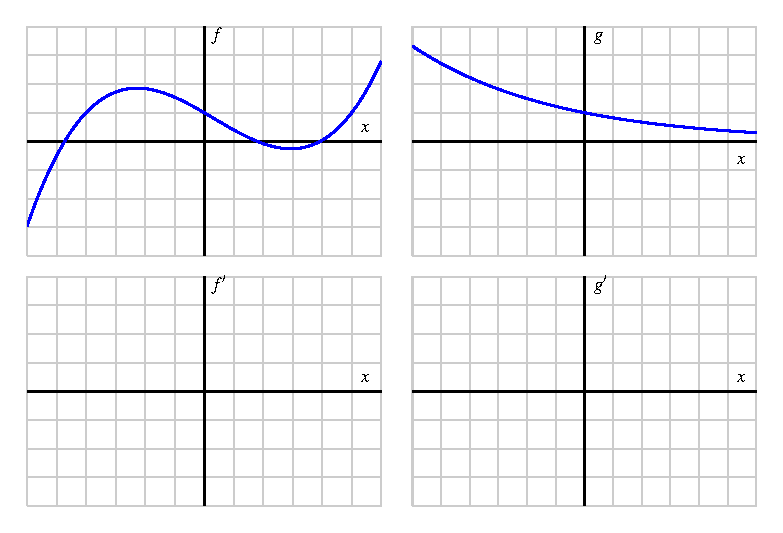
\includegraphics{figures/1_4_Act1a.eps}} 
%\centerline{\hspace{4in}}
\scalebox{0.85}{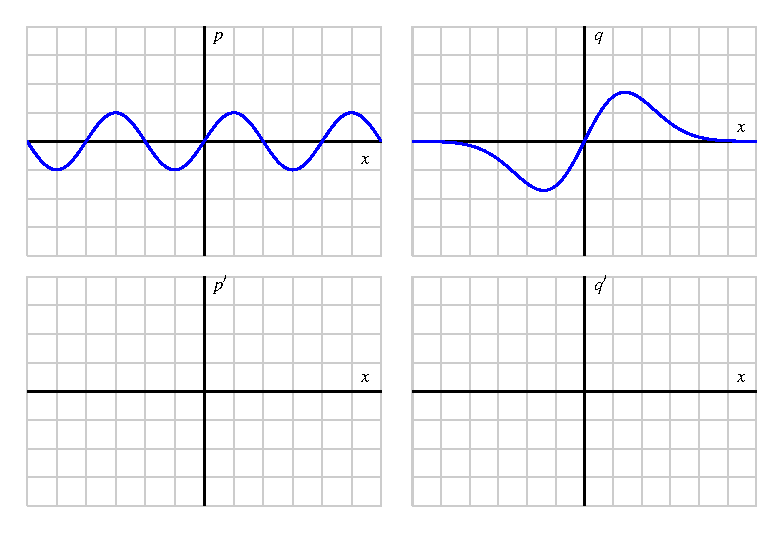
\includegraphics{figures/1_4_Act1b.eps}}
%\end{center}

\vfill \ \pagebreak

%\begin{center}
\scalebox{0.85}{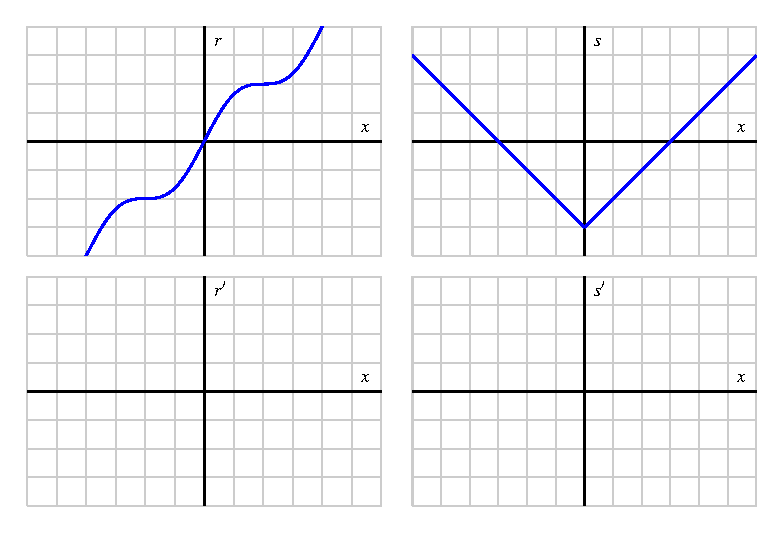
\includegraphics{figures/1_4_Act1c.eps}}
\centerline{\hspace{4in}}
\scalebox{0.85}{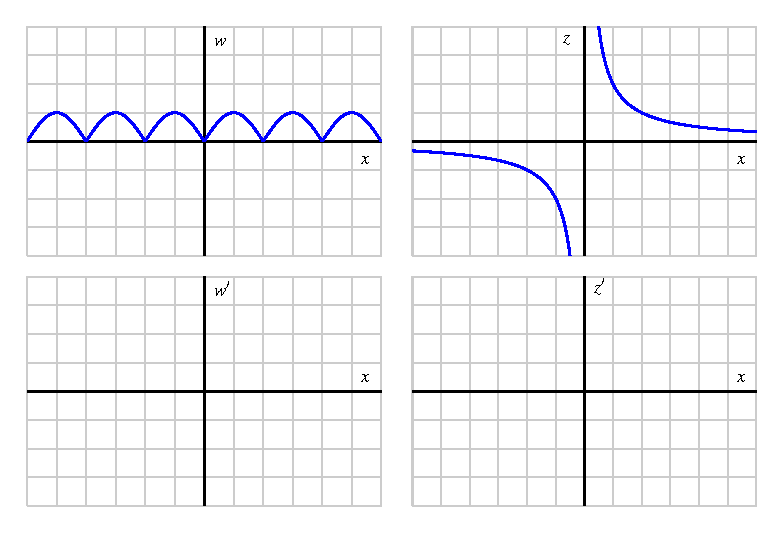
\includegraphics{figures/1_4_Act1d.eps}}
\end{center}

When you are finished with all 8 graphs, write several sentences that describe your overall process for sketching the graph of the derivative function, given the graph the original function.  What are the values of the derivative function that you tend to identify first?  What do you do thereafter?  How do key traits of the graph of the derivative function exemplify properties of the graph of the original function?

\end{activity}
\begin{smallhint}
Points where the slope of the tangent line is equal to zero are particularly important.  Try finding these points first in your effort to plot $y = f'(x)$ and plotting those zero values on the axes where you'll graph $y = f'(x)$.  
\end{smallhint}
\begin{bighint}
Points where the slope of the tangent line is equal to zero are particularly important.  Try finding these points first in your effort to plot $y = f'(x)$ and plotting those zero values on the axes where you'll graph $y = f'(x)$.  After doing so, think carefully as well about the questions: at this point, is $f'(x)$ positive or negative?  is $f'(x)$ big or small.  Use these ideas to help you sketch the derivative graph for the following functions.
\end{bighint}
\begin{activitySolution}
\begin{center}
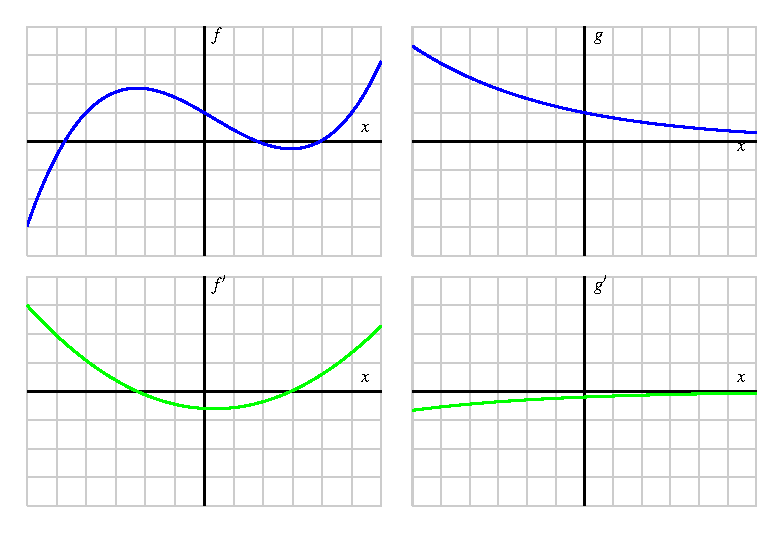
\includegraphics{figures/1_4_Act1aSoln.eps} \\
\underline{\hspace{4in}}\\
\ \\
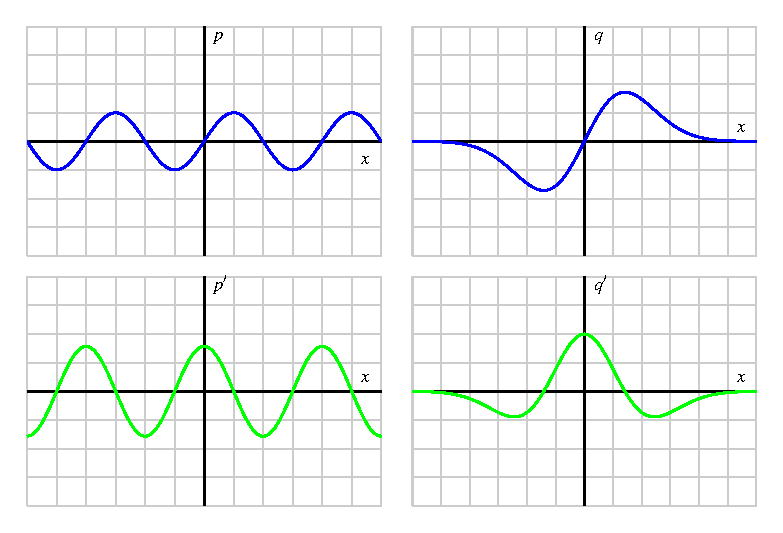
\includegraphics{figures/1_4_Act1bSoln.eps}
\end{center}

\begin{center}
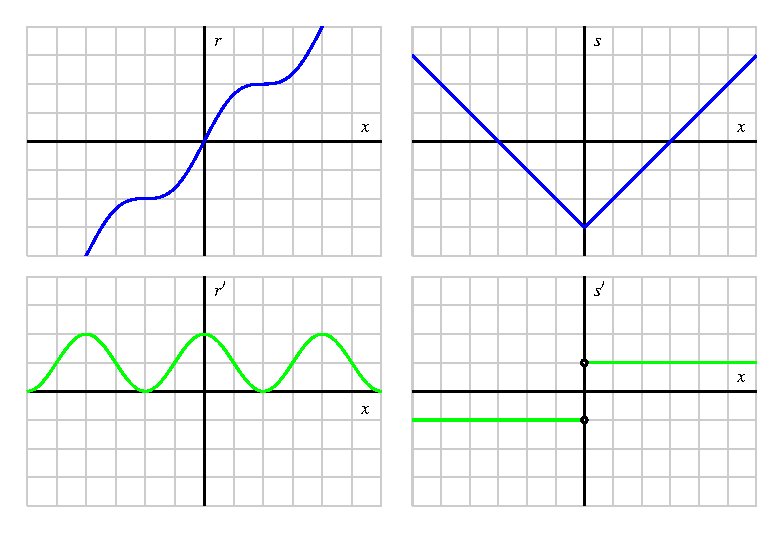
\includegraphics{figures/1_4_Act1cSoln.eps} \\
\underline{\hspace{4in}}\\
\ \\
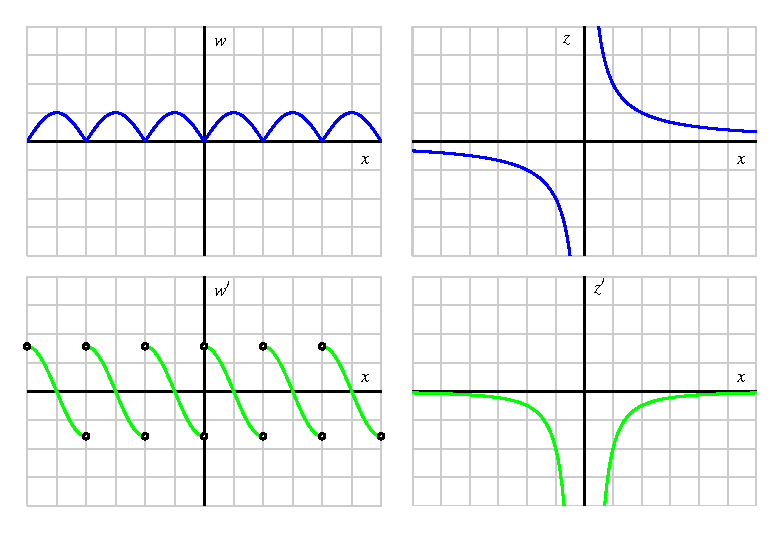
\includegraphics{figures/1_4_Act1dSoln.eps}
\end{center}
\end{activitySolution}
\aftera